\section*{dnešní elektronická varianta}
\addcontentsline{toc}{section}{dnešní elektronická varianta}

Čtvrtá elektronická varianta byla co se elektroniky týče přímým pokračováním předchozí verze. 
Hlavní dvě věci, co se změnili, bylo ovládání a princip zamykání. 

Princip mechanizmu
Zamykání je založeno na mechanizmu bajonetu a zamčení je zajištěno západkou, která zabraňuje zpětnému otočení.
Západka je ovládána motorem, který otáčí magnetem a tak přitahuje nebo odpuzuje magnet na západce. Důvodem pro magnetické ovládání
byla možnost západku ovládat i přes pevnou stěnu a také pružné spojení které takto vznikne, takže se trezor například dá zavřít i když
je už zamčen (když například dveře nejsou dovřeny).

\begin{figure}[htbp]
    \centering
    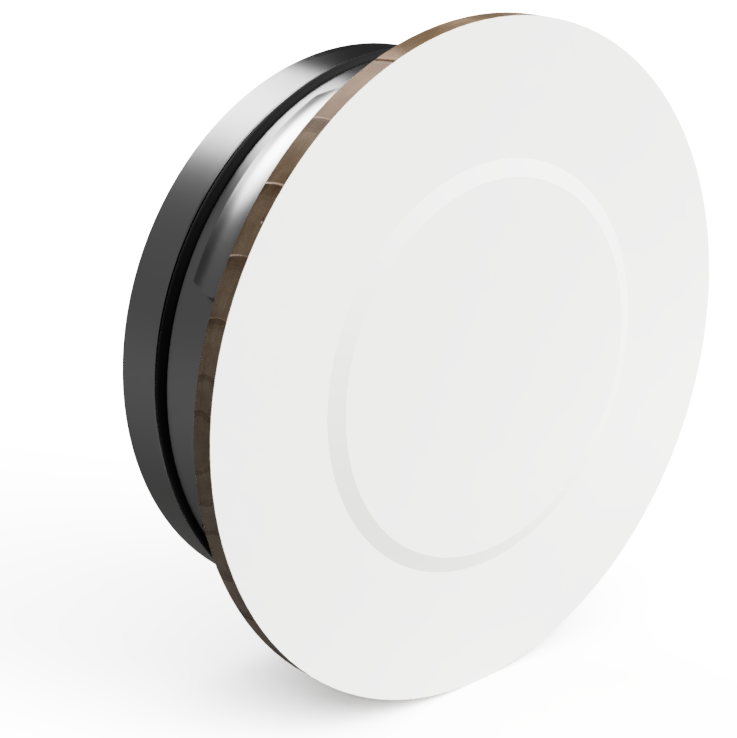
\includegraphics[width=170]{kapitoly/obrazky/E4/predni_render.png}
    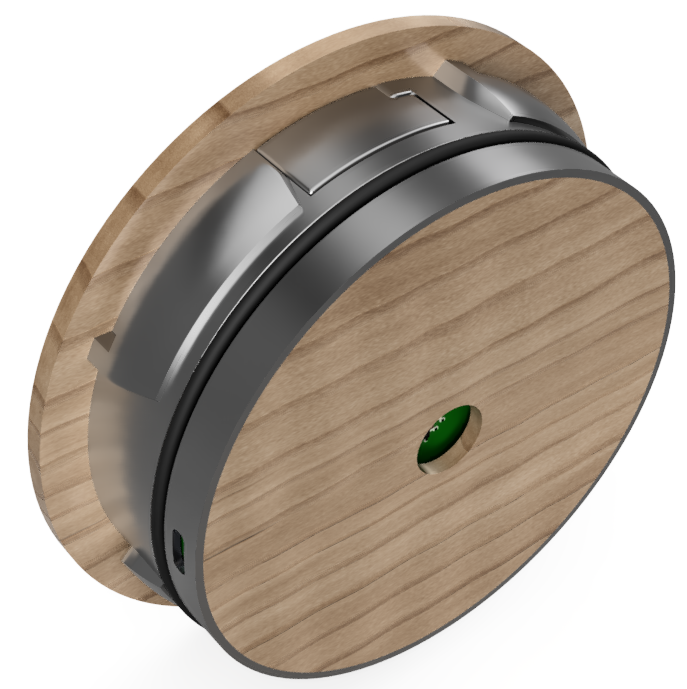
\includegraphics[width=170]{kapitoly/obrazky/E4/zadni_render.png}
    \label{fig:M1}
\end{figure}

\paragraph{Shrnutí změn z minulé verze}
Trezor získal možnost komunikace pomocí IR, pro možnost identifikace různých dveří, dále získal magnetický enkodér, pro možnost snazšího ovládání
motoru zámku. 
Další inovací byl programovací systém s USB-C, na místo USB-micro jako dřív. Tento programátor si má možnost úplně odpojit napájení, a to v rámci šetření 
energie, když ho trezor nevyužívá, a zároveň možnost zákazu přeprogramování.
Podstatnou změnou také bylo rozdělení elektroniky do dvou různých desek, protože na jedné by nebyl dostatek místa. Jedna deska tak obsahuje ledkový 
kruh a čip LDC1614 nebo LDC1314 se čtyřmi cívkami, které měří vzdálenost tlakové desky. Na druhé desce pak bylo vše ostatní, tedy procesor, akcelerometr,
gyroskop, magnetický kompas, RTC (Real Time Clock, hodiny reálného času), barometr, IR vysílač a přijímač, magnetický enkodér, programátor, řešení 
napájení, řízení motoru a nabíječka.

\subparagraph{Ovládání}
Předchozí varianty měli jako hlavní ovládací prvek enkodér s tlačítkem, ten jsem v nynější variantě odstranil, aby přední stěna neměla podobný velký 
výstupek. Proto jsem tento prvek nahradil indukční tlakovou deskou, která vyplnila vnitřek kruhu ledek. 
Zbytek ovládání víceméně přetrval, jen kvůli nedostatku času a pandemií způsobenému nedostatku součástek, trezor přišel o GPS. Na druhou stranu 
získal barometr s rozlišením schopným detekovat změnu výšky o půl metru.

\subparagraph{Napájení}
Předchozí verzím sloužila jako napájení powerbanka. Ta však kladla poměrné velké omezení, dokázala poskytnout proud pouze jedné ampéry, a proto 
jsem jí nahradil vlastním zdrojem, dvěma baterkami 18650. To však samozřejmě znamenalo nutnost vlastního řešení stabilizace napětí, díky čemuž 
trezor dostal stepup, který spíná napětí z 3.5V až 4.2V na 5V, a původně stepdown, později lineární stabilizátor, který poskytoval 3,3.5V.
Trezor také dostal vlastní nabíječku, aby stačilo připojit kabel, stejně jako třeba u mobilu.

\newpage